\documentclass[a4paper]{article}
\usepackage{geometry}                % See geometry.pdf to learn the layout options. There are lots.
\geometry{letterpaper}                   % ... or a4paper or a5paper or ... 
%\geometry{landscape}                % Activate for for rotated page geometry
%\usepackage[parfill]{parskip}    % Activate to begin paragraphs with an empty line rather than an indent
\usepackage{graphicx}
\usepackage{amssymb}
\usepackage{epstopdf}
\usepackage{multicol}
\usepackage{tikz}
\usetikzlibrary{calc}
\usepackage{mathptmx}

\DeclareGraphicsExtensions{.pdf,.png,.jpg}
\usepackage{wrapfig}

% Spacing stuff
\usepackage[cm]{fullpage}
\addtolength{\voffset}{-1in}
\setlength{\topmargin}{0pt}
\setlength\footskip{0pt}
\setlength{\parskip}{0cm}
\setlength{\parindent}{1em}
\usepackage[compact]{titlesec}
\titlespacing{\section}{0pt}{2ex}{1ex}
\titlespacing{\subsection}{5pt}{1ex}{2ex}
\titlespacing{\subsubsection}{0pt}{0.5ex}{0ex}

\title{Packing Game - Part A}
\author{
Donnie Smith (donnie.smith@gatech.edu) \\
Kyle Harrigan (kwharrigan@gmail.com) 
}	
\date{August 28, 2012}                                           % Activate to display a given date or no date

\begin{document}
\begingroup
\let\center\flushleft
\let\endcenter\endflushleft
\maketitle
\endgroup

\begin{tikzpicture}[remember picture,overlay]
  \node[anchor=north east,inner sep=0pt] at ($(current page.north east)-(1cm,0cm)$) {
     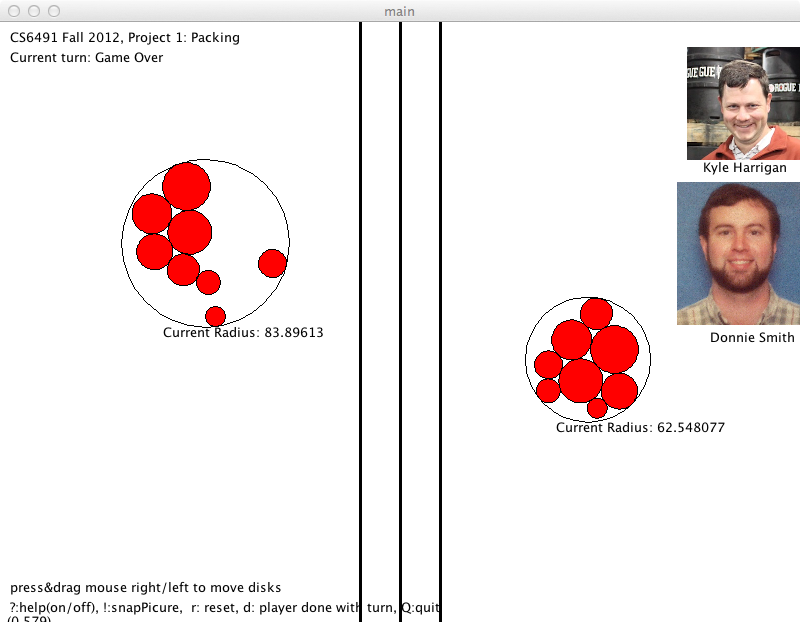
\includegraphics[width=300px,height=180px]{main/data/screenshot.png}

  };
\end{tikzpicture}


 \subsection{Problem Statement}
  
Implement an application which allows two human players to compete in an intense battle of disk packing.  The goal is for players to pack the disks as tightly as possible, resulting in the smallest enclosing sphere.  The program must calculate the minimal enclosing sphere, assign a score to each user, and declare a winner.  
 
 \subsection{Completed Features}
 \begin{multicols}{2}
 \begin{itemize}
 \setlength\multicolsep{0pt}
\itemsep0em 
\item Read disk count and disk sizes from file
\item Create initial holding area for discs
\item Limit disk movement to appropriate player's side
\item Implemented pairwise and triplet collision detection
\item Implemented bounding circles for pairs and triplets(minimal containing disk)
\item Implemented scoring and basic gameplay
\end{itemize}
\end{multicols}

 \subsection{To Be Done}
  \begin{multicols}{2}
 \begin{itemize}
\item Need to improve collision detection-- remove "flipping" and overlap conditions
\item Possibly optimize computation of minimal containing disk
\end{itemize}
\end{multicols}
 
\subsection{Computing Minimal Containing Disk}
The minimal containing circle was computed by finding the minimal containing circles for all pairs and some triplets of the circles.
The algorithm functions as follows:
\begin{enumerate}
	\item The current best solution is initialized to an impossibly large radius.
	\item For each pair of circles:
	\begin{enumerate}
		\item The minimum containing circle is computed.  If the radius of that circle is smaller than the current best solution:
		\begin{enumerate}
			\item If it contains all circles, then the current best solution is set to that circle.
			\item Otherwise, the minimal containing circle of all triplets that includes the initial pair are considered.  If that circle contains all circles:
			\begin{enumerate}
				\item If the circle is smaller than the current best solution, then the current best solution is set to that circle.
			\end{enumerate}
		\end{enumerate}
	\end{enumerate}
\end{enumerate}

This algorithm is not the most efficient available, but runs in $O(n^4)$ time, which is acceptable for a small number of circles.
The solution to the minimal bounding circle for triplets, which is one of the ten cases of Apollonius' Problem, was adapted from code written by Rasmus Fonseca.
The code was modified to fix a bug in which an invalid solution is found when two of the three circles are vertically aligned.

\subsection{Physics-Based AI Model}

\subsubsection*{Introduction}

Instead of a graph-based approach, we chose to employ a physics-based approach which models physics disks that move in a 2D plane.  Initially, disks are spread out in a circular pattern, and then a forcing function is applied at each update  

\subsubsection*{Initialization}
-Spread disks in circular pattern
(Picture)

\subsubsection*{Iterate}

-At each step, we compute the new the center of gravity
-For each disk, compute the velocity according to the forcing function (currently a velocity impulse)
  - Linear in the distance of the disk from the center of gravity
  - Quadratic in the radius of the disk
- Sort by increasing radius from the center of gravity
  - The purpose of this is to be able to detect all collisions with a single pass, as long as we can guarantee that no disk is moved towards the center of gravity as a result of collision detection
 - Compute the minimum bound, compare to the smallest seen minimum bound and if it is smaller record the disk configuration
  
\subsubsection*{Stopping Condition}
 - Currently fixed at 2000 iterations
  - Once the iterations are completed, we reset the configuration to the seen number of minimum disks
  
  





References:
\begin{itemize}
\itemsep0em
	\item http://en.wikipedia.org/wiki/Smallest\_circle\_problem
	\item http://mathworld.wolfram.com/ApolloniusProblem.html
	\item http://www.diku.dk/hjemmesider/ansatte/rfonseca/
	\item For handling multiple collisions (circle intersection problem) http://paulbourke.net/geometry/2circle/
\end{itemize}
\end{document}  
